\newpage
\section{Hình ảnh giao diện website}

\begin{figure}[htbp]
    \centering
    \includegraphics[width=0.85\textwidth]{static/banner2.webp}
    \caption[Giao diện trang chủ TimeLuxe]{Giao diện trang chủ website TimeLuxe. \protect\\
    Hiển thị banner chính với logo thương hiệu, thanh tìm kiếm và menu điều hướng. Thiết kế hiện đại với màu sắc sang trọng phù hợp với thương hiệu đồng hồ cao cấp.}
    \label{fig:homepage}
\end{figure}

\begin{figure}[htbp]
    \centering
    
\includegraphics[width=0.85\textwidth]{static/logo TIME LUXE.png}
    \caption[Logo thương hiệu TimeLuxe]{Logo chính của thương hiệu TimeLuxe. \protect\\
    Thiết kế logo thể hiện sự sang trọng và đẳng cấp, phù hợp với định vị thương hiệu đồng hồ cao cấp. Logo được sử dụng nhất quán trên toàn bộ website.}
    \label{fig:logo}
\end{figure}

\begin{figure}[htbp]
    \centering
    \includegraphics[width=0.85\textwidth]{static/dongho1.webp}
    \caption[Sản phẩm đồng hồ Citizen]{Sản phẩm đồng hồ Citizen Eco-Drive. \protect\\
    Hiển thị thông tin chi tiết sản phẩm bao gồm tên, giá, thương hiệu và hình ảnh chất lượng cao. Giao diện sản phẩm được thiết kế để tối ưu trải nghiệm mua sắm.}
    \label{fig:product}
\end{figure}

\begin{figure}[htbp]
    \centering
    \includegraphics[width=0.85\textwidth]{static/logo-citizen.png}
    \caption[Logo thương hiệu Citizen]{Logo thương hiệu Citizen. \protect\\
    Một trong những thương hiệu đồng hồ cao cấp được phân phối tại TimeLuxe. Website hỗ trợ hiển thị và lọc sản phẩm theo từng thương hiệu cụ thể.}
    \label{fig:citizen}
\end{figure}

\begin{figure}[htbp]
    \centering
    
\includegraphics[width=0.85\textwidth]{static/icon-shipping.png}
    \caption[Icon dịch vụ giao hàng]{Icon thể hiện dịch vụ giao hàng toàn quốc. \protect\\
    Website TimeLuxe cung cấp dịch vụ giao hàng miễn phí cho đơn hàng từ 500k, thể hiện cam kết về chất lượng dịch vụ khách hàng.}
    \label{fig:shipping}
\end{figure}

\begin{figure}[htbp]
    \centering
    
\includegraphics[width=0.85\textwidth]{static/icon-warranty.png}
    \caption[Icon bảo hành chính hãng]{Icon thể hiện chính sách bảo hành chính hãng. \protect\\
    TimeLuxe cam kết bảo hành chính hãng 5 năm và đổi trả trong 7 ngày, đảm bảo quyền lợi tối đa cho khách hàng.}
    \label{fig:warranty}
\end{figure}

\newpage
\section{Sơ đồ kiến trúc hệ thống}

\begin{figure}[htbp]
    \centering
    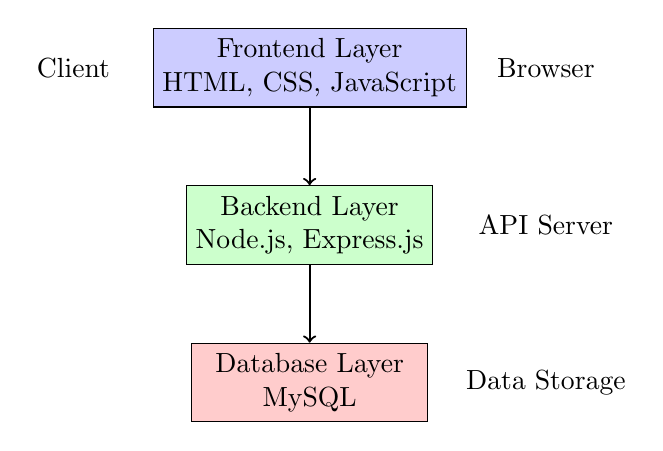
\begin{tikzpicture}[
        node distance=2cm,
        box/.style={rectangle, draw, minimum width=3cm, minimum height=1cm, align=center},
        arrow/.style={->, thick}
    ]
    
    % Frontend Layer
    \node[box, fill=blue!20] (frontend) {Frontend Layer\\HTML, CSS, JavaScript};
    
    % Backend Layer
    \node[box, fill=green!20, below of=frontend] (backend) {Backend Layer\\Node.js, Express.js};
    
    % Database Layer
    \node[box, fill=red!20, below of=backend] (database) {Database Layer\\MySQL};
    
    % Arrows
    \draw[arrow] (frontend) -- (backend);
    \draw[arrow] (backend) -- (database);
    
    % Labels
    \node[left of=frontend, xshift=-1cm] {Client};
    \node[right of=frontend, xshift=1cm] {Browser};
    \node[right of=backend, xshift=1cm] {API Server};
    \node[right of=database, xshift=1cm] {Data Storage};
    
    \end{tikzpicture}
    \caption[Kiến trúc 3-tier của hệ thống]{Kiến trúc 3-tier của website TimeLuxe. \protect\\
    Hệ thống được chia thành 3 lớp chính: Frontend (giao diện người dùng), Backend (xử lý logic nghiệp vụ), và Database (lưu trữ dữ liệu).}
    \label{fig:architecture}
\end{figure}

\newpage
\section{Sơ đồ cơ sở dữ liệu}

\begin{figure}[htbp]
    \centering
    \begin{tikzpicture}[
        node distance=2.5cm,
        entity/.style={rectangle, draw, minimum width=2.5cm, minimum height=1.5cm, align=center},
        relationship/.style={diamond, draw, minimum width=1.5cm, minimum height=1cm, align=center}
    ]
    
    % Entities
    \node[entity] (users) {Users\\(id, username, email, password, role)};
    \node[entity, right of=users] (products) {Products\\(id, name, brand, price, description)};
    \node[entity, below of=users] (orders) {Orders\\(id, user\_id, total\_amount, status)};
    \node[entity, below of=products] (order\_details) {Order\_Details\\(order\_id, product\_id, quantity, price)};
    \node[entity, below of=orders] (cart) {Cart\\(user\_id, product\_id, quantity)};
    
    % Relationships
    \node[relationship, right of=orders] (places) {places};
    \node[relationship, right of=order\_details] (contains) {contains};
    \node[relationship, below of=cart] (adds) {adds};
    
    % Lines
    \draw (users) -- (places);
    \draw (places) -- (orders);
    \draw (orders) -- (contains);
    \draw (contains) -- (order\_details);
    \draw (products) -- (contains);
    \draw (users) -- (adds);
    \draw (adds) -- (cart);
    \draw (products) -- (adds);
    
    \end{tikzpicture}
    \caption[ERD - Entity Relationship Diagram]{Sơ đồ quan hệ thực thể (ERD) của hệ thống. \protect\\
    Mô tả mối quan hệ giữa các bảng: Users (người dùng), Products (sản phẩm), Orders (đơn hàng), Order\_Details (chi tiết đơn hàng), và Cart (giỏ hàng).}
    \label{fig:erd}
\end{figure}

\newpage
\section{Luồng xử lý đơn hàng}

\begin{figure}[htbp]
    \centering
    \begin{tikzpicture}[
        node distance=2cm,
        process/.style={rectangle, draw, rounded corners, minimum width=2.5cm, minimum height=1cm, align=center},
        decision/.style={diamond, draw, minimum width=2cm, minimum height=1cm, align=center},
        start/.style={ellipse, draw, minimum width=2cm, minimum height=1cm, align=center},
        arrow/.style={->, thick}
    ]
    
    % Flow
    \node[start] (start) {Bắt đầu};
    \node[process, below of=start] (browse) {Duyệt sản phẩm};
    \node[process, below of=browse] (add) {Thêm vào giỏ hàng};
    \node[decision, below of=add] (check) {Kiểm tra đăng nhập?};
    \node[process, left of=check, xshift=-2cm] (login) {Đăng nhập};
    \node[process, below of=check] (checkout) {Thanh toán};
    \node[decision, below of=checkout] (payment) {Thanh toán thành công?};
    \node[process, left of=payment, xshift=-2cm] (retry) {Thử lại};
    \node[process, below of=payment] (confirm) {Xác nhận đơn hàng};
    \node[start, below of=confirm] (end) {Kết thúc};
    
    % Arrows
    \draw[arrow] (start) -- (browse);
    \draw[arrow] (browse) -- (add);
    \draw[arrow] (add) -- (check);
    \draw[arrow] (check) -- node[left] {Không} (login);
    \draw[arrow] (login) -- (check);
    \draw[arrow] (check) -- node[right] {Có} (checkout);
    \draw[arrow] (checkout) -- (payment);
    \draw[arrow] (payment) -- node[left] {Không} (retry);
    \draw[arrow] (retry) -- (checkout);
    \draw[arrow] (payment) -- node[right] {Có} (confirm);
    \draw[arrow] (confirm) -- (end);
    
    \end{tikzpicture}
    \caption[Luồng xử lý đơn hàng]{Luồng xử lý đơn hàng trong hệ thống TimeLuxe. \protect\\
    Mô tả quy trình từ việc duyệt sản phẩm đến hoàn thành đơn hàng, bao gồm các bước kiểm tra đăng nhập và xử lý thanh toán.}
    \label{fig:order-flow}
\end{figure}

\end{document} 